\documentclass[fleqn]{jbook}
\usepackage{physpub}

\begin{document}

\begin{question}{教育 物理}{}

% Definition of local macros
\def\PA{{\rm A}}
\def\PB{{\rm B}}
\def\PC{{\rm C}}


\begin{subquestions}
\SubQuestion
  長さ $2a$ で質量の無視できる剛体の棒の両端に、ともに質量 $M$ を
  もつ質点 \PA および \PB が取り付けられ、図のように $xy$
  平面内に静止している。
  そこに質量 $m$ の質点 \PC が、図のように直線 $y=a$ に沿って、
  速度 $v$ で $x$ 軸の正の向きに等速直線運動して、質点 \PA と
  衝突した。
  衝突は完全弾性的であり、衝突後の \PC の運動は $x$ 軸に平行
  であるとして、以下の設問に答えよ。ただし摩擦や重力は考えない。

  \parbox[t]{105mm}{
  \begin{subsubquestions}
  \SubSubQuestion
    衝突後の系 $(\PA,\PB,\PC)$ の運動を記述するのに適した
    複数個の物理量を定義し、それらがどのような力学的保存則
    により決定されるかを述べ、式で表せ。

  \SubSubQuestion
    力学的保存則を解いて、上で定義した物理量を、$M$、$m$、$a$、
    および $v$ で表せ。

  \SubSubQuestion
    衝突後、質点 \PA および \PB の速度の $x$ 成分は、どのよう
    に時間変化するか。衝突後の経過時間 $t$ の関数として、同一
    のグラフに図示せよ。特徴的な座標の値も記入すること。

  \end{subsubquestions}

  }\parbox[t]{55mm}{
  \vspace*{-5mm}\begin{center}
    \mbox{\includegraphics[clip]{1996phys-1.eps}}
  \end{center}}
  
\SubQuestion

  電荷 $q$、質量 $m$ の荷電粒子の位置ベクトルを 
  $\Vec{r}(t) = (x(t),y(t),z(t))$ で表す。
  粒子の速度は光速度と比べて\\十分小さいとして以下の設問に答えよ。


  \begin{subsubquestions}
  \SubSubQuestion
    一様な静磁場 $\Vec{B} =(0,0,B)$ がかかっているときの
    荷電粒子の運動sで、時刻 $t=0$ での初期条件 $\Vec{r} = (0,0,0)$、
    $\tDeriver{\Vec{r}}{t} = (v_0,0,u_0)$ を満たすものを求めよ。

  \SubSubQuestion
    上記静磁場と振動数 $\omega = qB/m$ をもつ電場 
    $\Vec{E} = (E\cos{\omega t},-E\sin{\omega t},0)$
    がかかっているとき、運動方程式の解で、時刻 $t=0$ での
    初期条件 $\Vec{r} = (0,0,0)$、$\tDeriver{\Vec{r}}{t}=(0,0,0)$ 
    を満たすものを求めよ。この場合、運動方程式は複素変数
    $\tDeriver{x}{t}+i\tDeriver{y}{t}$ を用いると扱いやすい。

  \SubSubQuestion
    前問について、運動エネルギー $K$ の変化率 $\tDeriver{K}{t}$ を
    求めよ。また、電場 $\Vec{E}$ と粒子の速度 $\Vec{v}$ 
    の関係に注目して、この結果を説明せよ。

  \end{subsubquestions}

\SubQuestion

  通常、気体は高温低密度の極限で理想気体に近づくが、一般には
  理想気体からのずれが観測される。
  このようなずれを示す気体1モルに対して、以下の設問に答えよ。

  \begin{subsubquestions}
  \SubSubQuestion
    この気体を体積 $V$ に保って熱容量を測定したところ、温度
    $T_1<T_2$ の間で、$C=2.5R-gT^{-2}$ と表されることがわかった。
    但し、$R$ は気体定数であり、$g$ は温度によらない定数である。
    この測定で、温度 $T_1$ から温度 $T_2$ まで気体の温度を上昇
    させたときの気体のエントロピーの増加量を求めよ。

  \SubSubQuestion
    熱膨張率 $\alpha$ と等温圧縮率 $\kappa$ を測定したところ、
    次のような関数で表されることがわかった。

    \vspace*{2mm}\begin{minipage}{75mm}
    \begin{equation}
      \alpha \equiv +\frac{1}{V} \Bigl( \Partial{V}{T} \Bigr) _p =
      \frac{1}{T} \Bigl( 1+\frac{a}{VT} \Bigr) \eqname{alpha}
    \end{equation}
    \end{minipage}\begin{minipage}{75mm}
    \begin{equation}
      \kappa \equiv -\frac{1}{V} \Bigl( \Partial{V}{p} \Bigr) _T =
      \frac{1}{p} \Bigl( 1+\frac{b}{VT} \Bigr) \eqname{kappa}
    \end{equation}
    \end{minipage}\vspace*{2mm}

    但し、$V$、$T$、$p$ はそれぞれの気体の体積、温度、圧力で
    ある。また、$a$、$b$ は同じ次元を持つ定数である。\\
    $V$ の2階偏導関数を考えることにより、$a=2b$ であることを
    証明せよ。

  \SubSubQuestion
    この気体の状態方程式を以下の順で求めよう。
    先ず式\eqhref{kappa}のみを用いて、等温過程における、
    $p$ と $V$ の関係を求めよ。
    次にこの結果を式\eqhref{alpha}に代入して、状態方程式
    を決定せよ。

  \end{subsubquestions}
\end{subquestions}
\end{question}
\begin{answer}{教育 物理}{}
% Definition of local macros
\def\PA{{\rm A}}
\def\PB{{\rm B}}
\def\PC{{\rm C}}

\begin{subanswers}
\SubAnswer

  \begin{subsubanswers}
  \SubSubAnswer
    \parbox[t]{95mm}{
    衝突後、2球 $\PA$と$\PB$ はその重心を$x$ 軸に平行に移動させながら
    重心を中心として回転運動を行う。
%
    衝突後の $\PC$ の速度を $v^\prime$ とする。
    衝突後の $\PA$と$\PB$の重心の速度を $V$ とし、
    重心を中心とする回転角速度を $\omega$ とする。

    衝突は瞬間的として $\PC$ が $\PA$ に及ぼす撃力を $J$ とする。
    $\PC$ は反作用として $\PA$ から撃力 $-J$ を受ける。

    運動量保存則より次の2式が成り立つ。
%
    }\parbox[t]{55mm}{\vspace*{-15mm}
    \begin{center}
      \mbox{\includegraphics[clip]{1996phys-2.eps}}
    \end{center}}
%
    \begin{eqnarray}
     mv - J &=& mv^\prime \eqname{C_moment}\\
          J &=& 2MV       \eqname{AB_moment}
    \end{eqnarray}
%
    また角運動量保存則より次の式が成り立つ。
%
    \begin{equation}
          aJ = 2Ma^2 \omega \eqname{AB_angulermoment}
    \end{equation}
%
    最後にエネルギー保存則より次の式が成り立つ。
%
    \begin{equation}
    \frac{1}{2} mv^2 = \frac{1}{2} mv^{\prime2} + \frac{1}{2} 2MV^2 + \frac{1}{2} 2Ma^2\omega^2  \eqname{Energy}
    \end{equation}
%
    以上4式がこの系を支配する保存則である。

  \SubSubAnswer
    式\eqhref{AB_moment}と式\eqhref{AB_angulermoment}より $a\omega=V$
    がわかる。これと式\eqhref{Energy}より$mv^2 - mv^{\prime2} = 4MV^2$
    となる。

    さらに式\eqhref{C_moment}と式\eqhref{AB_moment}より$mv-mv^\prime=2MV$
    がわかる。よって$v+v^\prime = 2V$となる。

    これらより次の諸量が求まる。
%
    \[ V=\frac{m}{m+M}v \hspace{15mm} v^\prime=\frac{m-M}{m+M}v \hspace{15mm} \omega=\frac{m}{m+M}\frac{v}{a} \]
%
  \SubSubAnswer
    衝突後の\PA と\PB の速度をそれぞれ $V_A$、$V_B$と表す。明らかに\\
    \parbox{70mm}{
      \begin{eqnarray*}
       V_A &=& V + a\omega{\cos\omega t} \\
           &=& \frac{m}{m+M}v\Bigl(1+\cos{\frac{m}{m+M}\frac{v}{a}t}\Bigr) 
      \end{eqnarray*}
    }
    \parbox{70mm}{
      \begin{eqnarray*}
       V_B &=& V - a\omega{\cos\omega t} \\
           &=& \frac{m}{m+M}v\Bigl(1-\cos{\frac{m}{m+M}\frac{v}{a}t}\Bigr)
      \end{eqnarray*}
    }\\
    これより$V_A$、$V_B$の時間変化は下図のようになる。
%
    \begin{center}
      \mbox{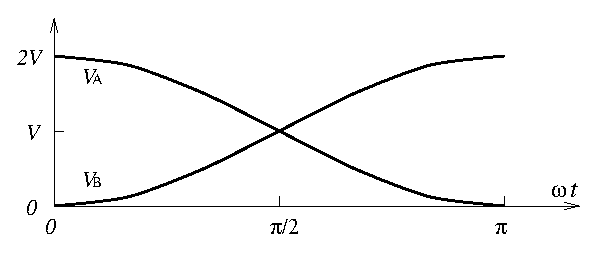
\includegraphics[clip]{1996phys-3.eps}}
    \end{center}
%



  \end{subsubanswers}

\SubAnswer
  \begin{subsubanswers}
  \SubSubAnswer
    運動方程式は $ m \ddot{\Vec{r}} = q \dot{\Vec{r}} \times \Vec{B}$
    である。成分ごとに表すと
%
    \[ \ddot{z} = 0 \hspace{10mm} %
       \ddot{x} = \frac{qB}{m} \dot{y} \hspace{10mm} %
       \ddot{y} = -\frac{qB}{m} \dot{x} \]
%
    ここで複素数 $w$ を $w=x+iy$ と定義すると上式は、
%
    \[ \ddot{z} = 0 \hspace{10mm} %
       \ddot{w} = -i \frac{qB}{m} \dot{w} \]
%
    となる。初期条件 $\dot{w}|_{t=0}=v_o$、$\dot{z}|_{t=0}=u_o$を
    考慮して積分すると、
%
    \[ \dot{z} = u_o \hspace{8mm} %
       \dot{w} = -i \frac{qB}{m} \left( w + i \frac{m}{qB} v_o\right)\]
%
    さらに、初期条件 $w|_{t=0}=0$、$z|_{t=0}=0$ 考慮して積分すると、
%
    \[ z = u_o t \hspace{7mm} %
       w = -i \frac{m}{qB} v_o\bigr( 1-e^{-i\frac{qB}{m}t} \bigl) \hspace{10mm} \]
%

    実数に直して求める荷電粒子の軌道が得られる。
%
    \[ z = u_o t \hspace{7mm} %
       x = \frac{m}{qB} v_o \sin{\frac{qB}{m}t} \hspace{10mm} %
       y = \frac{m}{qB} v_o \cos{\frac{qB}{m}t} - \frac{m}{qB} v_o \]
%
  \SubSubAnswer
    運動方程式は $ m \ddot{\Vec{r}} = q\Vec{E} + q \dot{\Vec{r}} \times \Vec{B}$
    である。成分毎に表すと
%
    \[ \ddot{z} = 0 \hspace{10mm} %
       \ddot{x} =   \frac{qE}{m}\cos{\omega t} + \frac{qB}{m} \dot{y} \hspace{10mm} %
       \ddot{y} = - \frac{qE}{m}\sin{\omega t} - \frac{qB}{m} \dot{x} \]
%
    ここで複素数 $w$ を $w=x+iy$ と定義すると上式は、
%
    \[ \ddot{z} = 0 \hspace{10mm} %
       \ddot{w} = \omega\frac{E}{B}e^{-i\omega t} -i \omega \dot{w} \]
%
    となる。初期条件 $\dot{w}|_{t=0}=0$、$\dot{z}|_{t=0}=0$を
    考慮して積分すると、
%
    \[ \dot{z} = 0 \hspace{10mm} %
       \dot{w}+ i \omega w = i\frac{E}{B}\bigl(e^{-i\omega t}-1\bigr) \]
%
    この $w$ に関する微分方程式は非斉次である。特殊解として次の形式の
    解を仮定する。
%
    \[ w = C_1 te^{-i\omega t} - \frac{E}{\omega B} \]
%
    これを微分方程式に代入して整理することにより $ C_1 =i E/B$ が
    求まる。

    次に斉次方程式の一般解として次の形式の解がある。
%
    \[ w = C_2 e^{-i\omega t} \]
%
    よって微分方程式の解は、初期条件 $w|_{t=0}=0$、$z|_{t=0}=0$ 
    考慮して
%
    \[ w = C_2 e^{-i\omega t} + i\frac{E}{B}te^{-i\omega t} - \frac{E}{\omega B} = i\frac{E}{\omega B}(1+i\omega t)e^{-i\omega t} - \frac{E}{\omega B} \]
%
    となる。実数にもどして
%
    \[ z = 0 \hspace{10mm}%
       x = \frac{E}{\omega B}(\cos{\omega t} + \omega t\sin{\omega t} ) - \frac{E}{\omega B} \hspace{10mm}%
       y = \frac{E}{\omega B}(-\sin{\omega t} + \omega t\cos{\omega t} ) \]
%
  \SubSubAnswer
    荷電粒子の複素速度 $\dot{w}$ は前問の結果より計算され
%
    \begin{equation}
      \dot{w} = \frac{qE}{m} t e^{-i\omega t} \eqname{dotw-E}
    \end{equation}
%
    である。よって運動エネルギー $K$ は
%
    \[ K = \frac{1}{2} m \Norm{\dot{w}}^2 = \frac{q^2E^2}{2m} t^2 \]
%
    その時間変化率は
%
    \[ \Deriver{K}{t} = \frac{q^2E^2}{m} t \]
%
    である。
    これは等加速運動をする物体の運動エネルギーの変化の仕方と同じ
    である。式\eqhref{dotw-E}より荷電粒子の速度 $\Vec{v}$ は
    電場 $\Vec{E}$と常に平行であることがわかる。また、その速さ $v$ は
%
    \[ v = \frac{qE}{m} t \]
%
    であることより、電場による加速が等加速であることがわかる。つまり
    粒子は前問で求められた軌道にそって等加速運動を行うのである。
    その結果運動エネルギーは先に求められたように時間変化するのである。
  \end{subsubanswers}



\SubAnswer
% Definition of local macros
\def\Fixed#1#2{\left(#1\right)_{#2}}
% ---- 2階偏微分
\def\PartialII#1#2#3{\frac{\partial^2 #1}{\partial #2 \partial #3}}


  \begin{subsubanswers}
  \SubSubAnswer
    エントロピーの定義より、その増加量 $\IDelta S$ は
%
    \[ \IDelta S = \int_{T_1}^{T_2} \frac{\d{Q}}{T} \]
%
    で定義される。また、$\d{Q} = C \d{T}$であり
    問題の設定より $C = 2.5R - gT^{-2}$ であるので結局 $\IDelta S$ は
%
    \[ \IDelta S = \int_{T_1}^{T_2} \Bigl( \frac{2.5R}{T} - \frac{g}{T^3} \Bigr) \d{T} = 2.5R \log{\frac{T_2}{T_1}} + \frac{g}{2} \Bigl( \frac{1}{T_2^2}-\frac{1}{T_1^2} \Bigr) \]
%
    と求まる。

  \SubSubAnswer
    式 \eqhref{alpha} の両辺を $T$ を一定にしながら $p$ で偏微分する。
%
    \[ \Partial{}{p} \Fixed{\frac{1}{V} \Fixed{\Partial{V}{T}}{p}}{T} = \Partial{}{p} \Fixed{\frac{1}{T} + \frac{a}{VT^2}}{T} \]
%
    \begin{equation}
      \Yueni - \frac{1}{V^2} \Fixed{\Partial{V}{p}}{T} \Fixed{\Partial{V}{T}}{p} +  \frac{1}{V} \PartialII{V}{p}{T} = -\frac{a}{V^2T^2} \Fixed{\Partial{V}{p}}{T} = \frac{a}{pVT^2} \Bigl( 1 + \frac{b}{VT} \Bigr) \eqname{alpha2} 
    \end{equation}
%
    同様に式 \eqhref{kappa} の両辺を $p$ を一定にしながら $T$ で偏微分する。
%
    \[ \Partial{}{T} \Fixed{-\frac{1}{V} \Fixed{\Partial{V}{p}}{T}}{p} = \Partial{}{T} \Fixed{\frac{1}{p} + \frac{b}{pVT}}{p} \]
%
    \begin{eqnarray}
      \Yueni + \frac{1}{V^2} \Fixed{\Partial{V}{T}}{p} \Fixed{\Partial{V}{p}}{T} -  \frac{1}{V} \PartialII{V}{T}{p} = -\frac{b}{pV^2T} \Fixed{\Partial{V}{T}}{p} - \frac{b}{pVT^2} = -\frac{b}{pVT^2} \Bigl( 2 + \frac{a}{VT} \Bigr) \eqname{kappa2} 
    \end{eqnarray}
%
    式 \eqhref{alpha2}と 式 \eqhref{kappa2}の両辺を足すことで
    次の関係を得る。
%
    \[ a \Bigl( 1 + \frac{b}{VT} \Bigr) = b \Bigl( 2 + \frac{a}{VT} \Bigr) \hspace{20mm} \Yueni a = 2b \]
%

  \SubSubAnswer
    式 \eqhref{kappa} の $T$ を定数とみなして偏微分を常微分に置き換えて変形すると、
%
    \[ \frac{\d{V}}{V+b/T} = - \frac{\d{p}}{p} \hspace{20mm} \Yueni V = - \frac{b}{T} + \frac{C_1(T)}{p} \]
%
    ここで $C_1(T)$は $p$に依存しない $T$のある関数である。\\
    この $V$の表式を 式 \eqhref{alpha} に代入して整理すると
%
    \[ \Deriver{C_1(T)}{T} = \frac{C_1(T)}{T} \hspace{20mm} \Yueni C_1(T) = C_2 T \]
%
    ここで $C_2$ はある定数である。\\
    これらより気体の状態方程式は
%
    \[ V = - \frac{b}{T} + \frac{C_2T}{p} \]
%
    であるが、$b\to 0$の極限でこの気体は理想気体となる境界条件を
    課すことで $C_2=R$ がわかる。よって、
%
    \[ V = - \frac{b}{T} + \frac{RT}{p} \]
%
  \end{subsubanswers}
\end{subanswers}
\end{answer}


\end{document}
